\chapter[Visual Tokens and Visual Encoders]{Visual Tokens and Visual Encoders: Turning Images into Sequences}
\label{ch:visual-tokens-encoders}
\raggedbottom

Consider a common failure mode in VLM evaluation. A model describes a dining table scene fluently---naming plates, glasses, and a fruit bowl---while consistently getting wrong the color of a small cup near the left edge. The original photograph is several thousand pixels wide, but the model receives a resized input only a few hundred pixels across. After resizing and patching, the cup may shrink to a sliver smaller than a single patch, and the left margin may be represented mostly as tablecloth texture. One plausible explanation is not language-prior hallucination but encoding failure: the relevant cup evidence may never have reached the language model clearly enough to support the answer.

Part~IV ended with a systems audit. When an agent system succeeds, Chapter~\ref{ch:evaluating-model-systems} asked what the runtime actually improved: exposure, orchestration, delegation, stabilization, and efficiency under cost. Part~V changes the evidence type. The system is no longer only reading text, retrieved documents, tool outputs, or traces. It must process visual evidence.

This chapter studies the first bottleneck in that process:

\begin{quote}
A Transformer consumes sequences. An image is a continuous two-dimensional signal. How do we turn one into the other?
\end{quote}

\paragraph{Chapter thesis.} \emph{A VLM does not see pixels directly. It sees a budgeted, compressed, learned tokenization of pixels. Patch size, resolution, pooling, encoder architecture, and token selection decide which visual evidence survives. Many later multimodal failures begin before language generation, because the relevant evidence was never represented clearly enough in the visual tokens.}

\paragraph{What this chapter is not.} This is not a general history of computer vision. It is not a CLIP chapter; image-text contrastive alignment belongs to Chapter~\ref{ch:cross-modal-alignment}. It is not a VLM interface chapter; projectors, Q-Formers, cross-attention, visual prefixes, and interleaved tokens belong to Chapter~\ref{ch:visual-language-interface}. It is not a document understanding, OCR, GUI, or video chapter. Those settings will matter later, but this chapter focuses on a single question: how a still image becomes a finite set of visual tokens.

\paragraph{Running example.} Keep one image in mind: a table scene with a small cup on the left. The user asks, ``What color is the small cup on the left side of the table?'' A human looking at the original image can answer. A model may fail because the image was downsampled, the cup was smaller than a patch, the patch mixed cup and table, pooled features preserved only the scene gist, or token pruning removed the left-side detail. The rest of the chapter asks: \emph{did the visual evidence survive tokenization?}

\subsection*{Learning Objectives}

After completing this chapter, you should be able to:

\begin{enumerate}
  \item Explain why image tokenization is different from text tokenization.
  \item Compute the number of visual tokens produced by a patch-based encoder at a given resolution and patch size.
  \item Describe how a Vision Transformer turns image patches into token sequences.
  \item Distinguish local patch features, pooled image representations, and multiscale visual features.
  \item Explain the tradeoff between resolution, patch size, visual detail, compute, and context budget.
  \item Compare supervised, masked-image, and self-supervised visual encoder pretraining at a conceptual level.
  \item Identify encoding-layer failure modes such as small-object loss, attribute loss, pooling loss, and spatial precision loss.
  \item Design simple diagnostics to determine whether a VLM failure originated in visual encoding.
\end{enumerate}

\subsection*{Notation}

\begin{center}
\begin{tabularx}{\textwidth}{@{}lX@{}}
\toprule
Symbol & Meaning \\
\midrule
$I$ & Input image \\
$H, W$ & Image height and width in pixels \\
$C$ & Number of image channels \\
$P$ & Patch size, usually a square $P \times P$ region \\
$N_v$ & Number of visual tokens produced from an image \\
$d_v$ & Visual token dimension \\
$f_v$ & Visual encoder \\
$V = f_v(I)$ & Visual token sequence or representation \\
$v_i$ & The $i$-th visual token \\
$r$ & Image resolution scale or resized input resolution \\
$B_v$ & Visual token budget available to a downstream system \\
$\operatorname{crop}(I,\rho)$ & Crop of image $I$ at region $\rho$ \\
\bottomrule
\end{tabularx}
\end{center}

\subsection*{Timeline of Key Contributions}

\begin{center}
\begin{tabularx}{\textwidth}{@{}lX@{}}
\toprule
\textbf{Year} & \textbf{Milestone} \\
\midrule
2012 & AlexNet-era deep CNNs make learned visual features central to modern computer vision~\cite{krizhevsky2012imagenet}. \\
2015 & ResNets show that very deep residual visual encoders can scale effectively~\cite{he2016deep}. \\
2020 & The Vision Transformer formulates images as patch-token sequences processed by Transformers~\cite{dosovitskiy2020image}. \\
2021 & Swin Transformer introduces hierarchical, windowed attention for locality and resolution tradeoffs~\cite{liu2021swin}. \\
2021--2022 & BEiT and MAE make masked image modeling a major vision-side pretraining paradigm~\cite{bao2021beit,he2022masked}. \\
2022 & ConvNeXt shows that CNN and Transformer design ideas continue to cross-pollinate~\cite{liu2022convnet}. \\
2023 & DINOv2 provides strong general-purpose vision-only features for downstream tasks~\cite{oquab2023dinov2}. \\
2023 & Segment Anything highlights dense, region-aware visual representations and mask-level evidence~\cite{kirillov2023segment}. \\
2024--2026 & High-resolution, dynamic-resolution, and token-compressed VLM encoders make visual token budget a central systems constraint. \\
\bottomrule
\end{tabularx}
\end{center}

\paragraph{What this chapter covers.} We begin by separating image measurements from text tokens. We then explain the patch-embedding pipeline that makes images look like Transformer sequences, including positional information and the CNN-to-ViT shift. The middle of the chapter studies what visual encoders learn, how vision-only pretraining shapes those representations, and why resolution and token budget are not free knobs. The final sections turn visual tokenization into an audit framework: what details survive, what details are lost, and how to diagnose whether a VLM failure began before the language model.


%----------------------------------------------------------------------
\section{Images Are Not Text Tokens}
\label{sec:ch23-images-not-text}

Text tokenization begins with symbols. Visual tokenization begins with measurements.

A word such as \texttt{cup} is already a compact semantic unit. It points toward an object category, can be composed with adjectives, and participates in syntax. A subword token may be less meaningful than a word, but it still comes from a human writing system. Pixels are different. A pixel records a measurement at a location. A $16 \times 16$ image patch records 256 spatial measurements per channel. It may contain half of a cup, a strip of table, background texture, printed text, a specular highlight, or nothing the task cares about.

This difference is the first reason multimodal modeling is not just language modeling with another vocabulary. A language token sequence is already ordered, discrete, and designed for communication. An image is continuous-valued, two-dimensional, locally redundant, scale-sensitive, and task-dependent. Which part matters may not be the largest, most central, or most semantically common part of the scene.

\subsection{The Ambiguity of a Visual Token}

Suppose the small cup in the running example occupies a narrow region on the left side of the table. A patch-token system must decide how to represent the image before it knows the user's question. If the question asks for the room type, the cup is irrelevant. If the question asks for the cup color, the cup is central. If the question asks whether the cup is left of the plate, the spatial relation matters. The same pixels support different tasks.

This is why patch tokens are not visual words. A patch boundary can cut through an object. A patch can mix foreground and background. A token can encode texture but not object identity, or scene category but not color. Later layers can combine patches, but the initial discretization already sets a budget and a granularity.

\begin{tcolorbox}[colback=blue!5, colframe=blue!40, title=\textbf{Visual Tokens Are Not Words}]
A text token often corresponds to a word, subword, or punctuation mark. A visual token usually corresponds to a region of space after resizing and patching. It may contain:
\begin{itemize}[nosep,leftmargin=1.5em]
  \item part of one object;
  \item multiple objects;
  \item object plus background;
  \item text fragments or fine texture;
  \item a region that is irrelevant for the current task.
\end{itemize}
The token becomes useful only after a learned encoder turns local measurements into features.
\end{tcolorbox}

\subsection{The First Audit Question}

Part~IV taught an evidence audit for text systems: did the system expose the right paragraph, tool output, memory, or trace? The visual analogue is:

\begin{quote}
Did the visual evidence survive tokenization?
\end{quote}

If the answer is no, later stages cannot fix the failure by reasoning harder. The model can be well aligned, well instructed, and carefully prompted, while still missing the cup color because the relevant signal was never represented clearly enough. Chapter~\ref{ch:grounding-binding-visual-reasoning} will later ask whether the system bound ``red'' to ``cup'' rather than to another object. Chapter~\ref{ch:visual-language-interface} will ask whether visual tokens reached the language model effectively. This chapter asks the prior question: were the tokens good enough to contain the evidence?

\begin{quickrecap}
\textbf{Quick Recap.}
\begin{itemize}[nosep,leftmargin=1.5em]
  \item Text tokens start from symbols; visual tokens start from spatial measurements.
  \item A patch token is not naturally a semantic unit. It may mix objects, background, texture, and irrelevant detail.
  \item The first VLM audit question is whether task-relevant visual evidence survived tokenization.
\end{itemize}
\textit{Next: the Vision Transformer gives a simple, influential recipe for turning an image into a sequence.}
\end{quickrecap}


%----------------------------------------------------------------------
\section{Patch Embeddings and the ViT View}
\label{sec:ch23-patch-embeddings-vit}

The Vision Transformer made the image-to-sequence recipe explicit~\cite{dosovitskiy2020image}. Start with an image $I$ of shape $H \times W \times C$. Divide it into non-overlapping patches of size $P \times P$. Flatten each patch into a vector. Project that vector into a $d_v$-dimensional embedding. Add positional information. Feed the resulting sequence into Transformer blocks.

\begin{figure}[t]
\centering
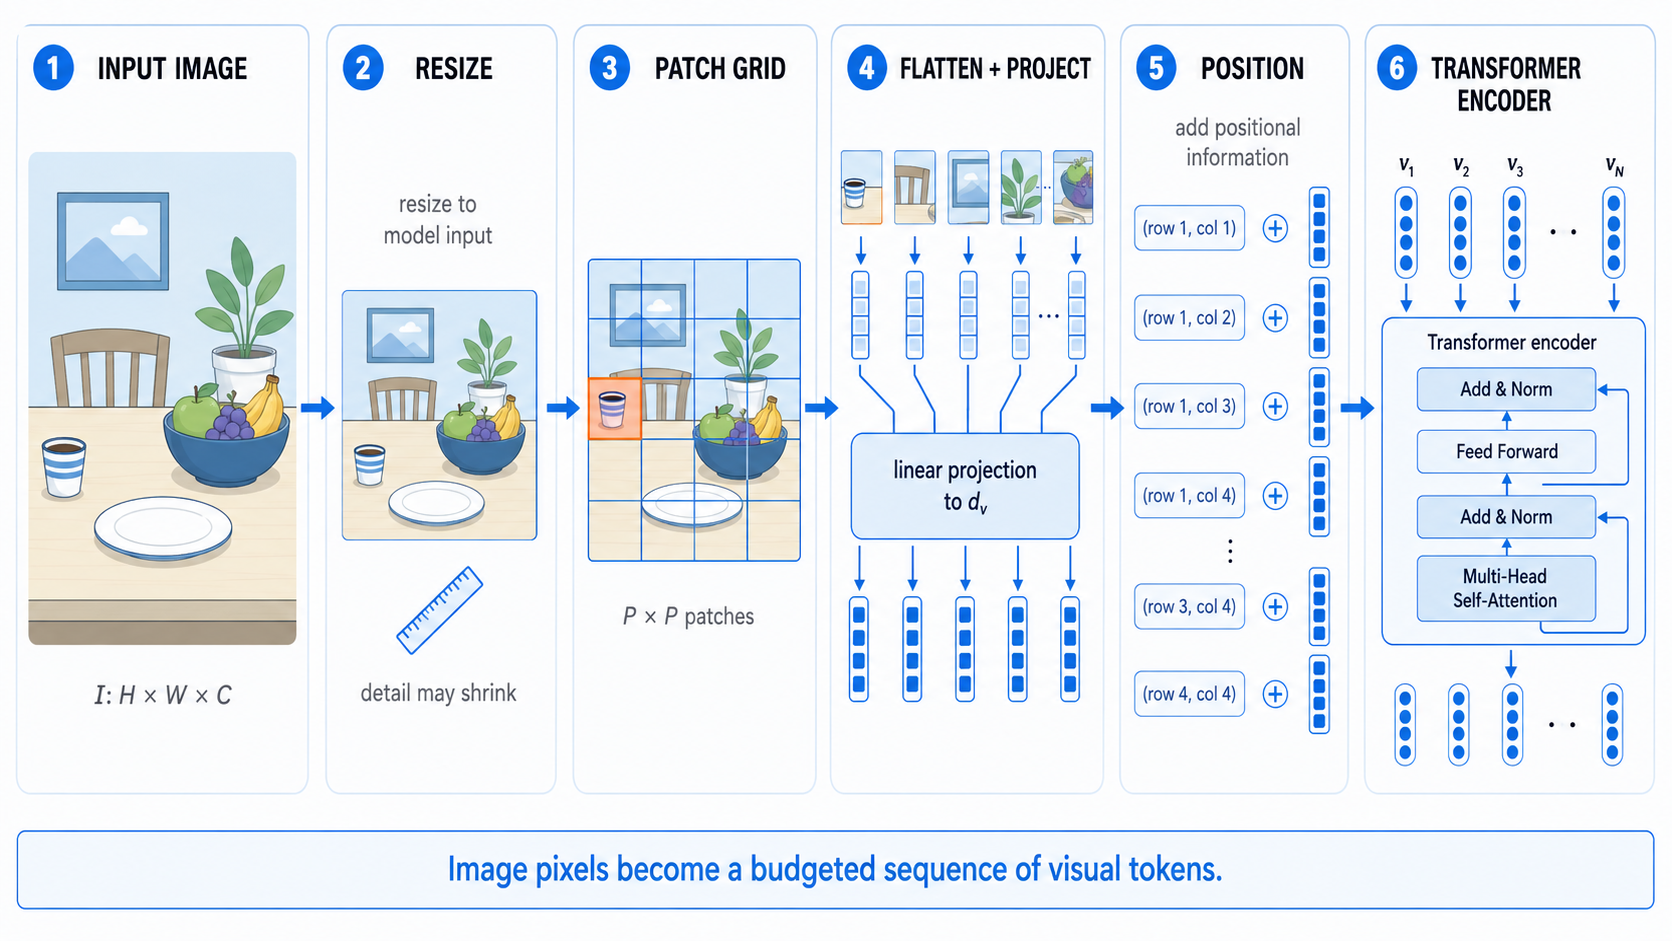
\includegraphics[width=0.96\textwidth]{figures/ch23/fig_image_to_visual_tokens.png}
\caption{\textbf{From image to visual tokens.} A patch-based encoder resizes the image, divides it into spatial patches, linearly projects each patch into a vector, adds position information, and processes the resulting sequence with Transformer blocks.}
\label{fig:ch23-image-to-visual-tokens}
\end{figure}

\subsection{The Hidden Tokenizer: Resize, Crop, Pad, Normalize}

Before patching begins, an image processor has already made important choices. It may resize the image to a fixed square, preserve aspect ratio and pad the empty region, center-crop the image, tile it, limit maximum pixels, interpolate between pixel grids, and normalize channels. These operations are part of visual tokenization, even though they happen before the Transformer sees a patch.

For the small-cup example, the first loss may occur here. If a wide photograph is squeezed or center-cropped into a standard input size, the left-side cup may become tiny, blurred, or excluded. That is not a failure of language reasoning, and it is not only a ViT patch-size problem. It is a preprocessing decision that determines which version of the image the encoder receives.

\subsection{Counting Visual Tokens}

For square images and square patches, the token count is:

\[
N_v = \frac{H}{P} \times \frac{W}{P}.
\]

This is the clean case. In practice, images may be resized, padded, tiled, or rounded so that the patch grid is valid. The formula still gives the basic budget intuition: tokens grow with image area and shrink with patch area.

If $H = W = 224$ and $P = 16$, the image becomes:

\[
N_v = 14 \times 14 = 196
\]

visual tokens. If $H = W = 448$ and $P = 16$, the image becomes:

\[
N_v = 28 \times 28 = 784.
\]

Doubling resolution quadruples the number of visual tokens. This is the first systems lesson of Part~V. Higher resolution may preserve small details, but it also increases attention cost, memory use, and the visual-token budget consumed by the image.

\begin{tcolorbox}[colback=blue!5, colframe=blue!40, title=\textbf{Token Count vs. Attention Cost}]
For fixed patch size:
\[
\text{resolution }2\times\text{ per side}
\;\rightarrow\;
\text{visual tokens }4\times
\;\rightarrow\;
\text{dense encoder attention pairs }\approx 16\times.
\]
If visual tokens directly enter an LLM context, downstream context pressure also grows. If they pass through pooling, token selection, a Q-Former, or another interface, fewer tokens may reach the LLM. Chapter~\ref{ch:visual-language-interface} studies that bridge; this chapter tracks the encoder-side cost of representing or selecting from the evidence.
\end{tcolorbox}

\begin{tcolorbox}[colback=blue!5, colframe=blue!40, title=\textbf{Pause and Verify}]
A $336 \times 336$ image is encoded with $14 \times 14$ patches. How many visual tokens are produced?

\medskip
\noindent\textbf{Answer.}
\[
\frac{336}{14} \times \frac{336}{14} = 24 \times 24 = 576.
\]
\end{tcolorbox}

\subsection{How Visual Tokens Know Where They Are}

A patch embedding alone says what local measurements are present. It does not say where the patch came from. Visual Transformers therefore add positional information: learned two-dimensional position embeddings, sinusoidal or relative variants, rotary-style schemes in some architectures, or position encodings adapted to windows and multiscale features.

Position matters more visibly for images than for many text examples. The answer to ``the cup on the left'' depends on location. If a model was trained at $224 \times 224$ with a $14 \times 14$ patch grid and later used at $448 \times 448$ with a $28 \times 28$ grid, the position embeddings may need interpolation. That interpolation is usually reasonable, but it is not magic. Resolution changes can alter how the model represents location, object size, and spatial relations.

This is one reason high-resolution evaluation should not only report final accuracy. It should also ask whether the architecture and positional scheme were designed for the new grid. A model can receive more pixels while still handling position poorly.

\subsection{Why Transformer-Compatible Vision Mattered}

CNN-style encoders such as AlexNet and ResNet learn powerful hierarchical features with local inductive bias and translation-friendly computation~\cite{krizhevsky2012imagenet,he2016deep}. Their feature maps can be connected to language systems, and modern CNNs remain important. But their native representation is a hierarchy of spatial maps, not a sequence that looks like language tokens.

ViT-style encoders made a different representation convenient: image patches become a sequence. This did not matter only because ViTs became strong classifiers. It mattered because images became easier to connect to Transformer machinery: attention, sequence batching, token selection, cross-attention, and downstream language interfaces. Swin-style models added hierarchy and windowed attention to improve locality and resolution scaling~\cite{liu2021swin}; ConvNeXt showed that CNNs could absorb many Transformer-era design lessons~\cite{liu2022convnet}. The practical lesson for VLMs is format as much as accuracy:

\begin{quote}
Vision Transformers made images look like sequences.
\end{quote}

\begin{quickrecap}
\textbf{Quick Recap.}
\begin{itemize}[nosep,leftmargin=1.5em]
  \item A patch encoder maps an $H \times W \times C$ image into $N_v$ visual tokens.
  \item For patch size $P$, $N_v = (H/P)(W/P)$, so resolution increases token count quadratically.
  \item Positional information is essential because visual tokens need spatial coordinates, not only local content.
  \item ViT-style encoders mattered because they made image representations naturally Transformer-compatible.
\end{itemize}
\textit{Next: once the image is a sequence, the encoder still has to decide what visual features to preserve.}
\end{quickrecap}


%----------------------------------------------------------------------
\section{What a Visual Encoder Learns}
\label{sec:ch23-what-encoder-learns}

We can write a visual encoder as:

\[
V = f_v(I),
\]

where $V$ may be a sequence of patch-level features, a pooled global representation, a CLS token, multiscale feature maps, region features, or a compressed token set. The important point is that $V$ is not the image. It is a learned representation of the image.

\begin{center}
\small
\begin{tabularx}{\textwidth}{@{}p{3.0cm}p{5.6cm}X@{}}
\toprule
\textbf{Term} & \textbf{Meaning} & \textbf{Risk} \\
\midrule
Patch token & Fixed spatial patch embedding before or early in the encoder & Object cut by patch boundary; mixed background \\
Encoder token & Contextualized patch feature after visual Transformer layers & Local detail may blur or become entangled \\
Pooled token / CLS & Global summary of the image or feature sequence & Local evidence may be lost \\
Region token & Object, mask, proposal, or crop-level feature & Depends on detector, segmenter, or crop policy \\
Compressed token & Selected, merged, pooled, or resampled visual information & Task-relevant detail may be dropped \\
\bottomrule
\end{tabularx}
\end{center}

When this chapter says ``visual token,'' it means this family of learned visual representations, not one uniform object.

\subsection{Local Features and Global Features}

Local features preserve information tied to regions: small objects, colors, textures, boundaries, text fragments, instance locations, and spatial relations. They matter for questions like:

\begin{itemize}[nosep,leftmargin=1.5em]
  \item What color is the small cup?
  \item Is the spoon to the left of the plate?
  \item How many blue markers are on the desk?
  \item What word is printed on the sign?
\end{itemize}

Global features summarize the whole image: scene category, overall gist, image-level retrieval identity, coarse caption, or class label. They matter for questions like:

\begin{itemize}[nosep,leftmargin=1.5em]
  \item Is this image indoors or outdoors?
  \item Does the image contain a dining table?
  \item Which caption best matches the image?
\end{itemize}

A representation can be excellent for global matching and weak for local grounding. A pooled embedding may know ``kitchen table with cups'' while losing the color of the small left cup. This distinction prepares Chapter~\ref{ch:cross-modal-alignment}: image-text alignment can make global embeddings useful for retrieval, but global alignment does not guarantee local evidence is preserved for every question.

\begin{figure}[t]
\centering
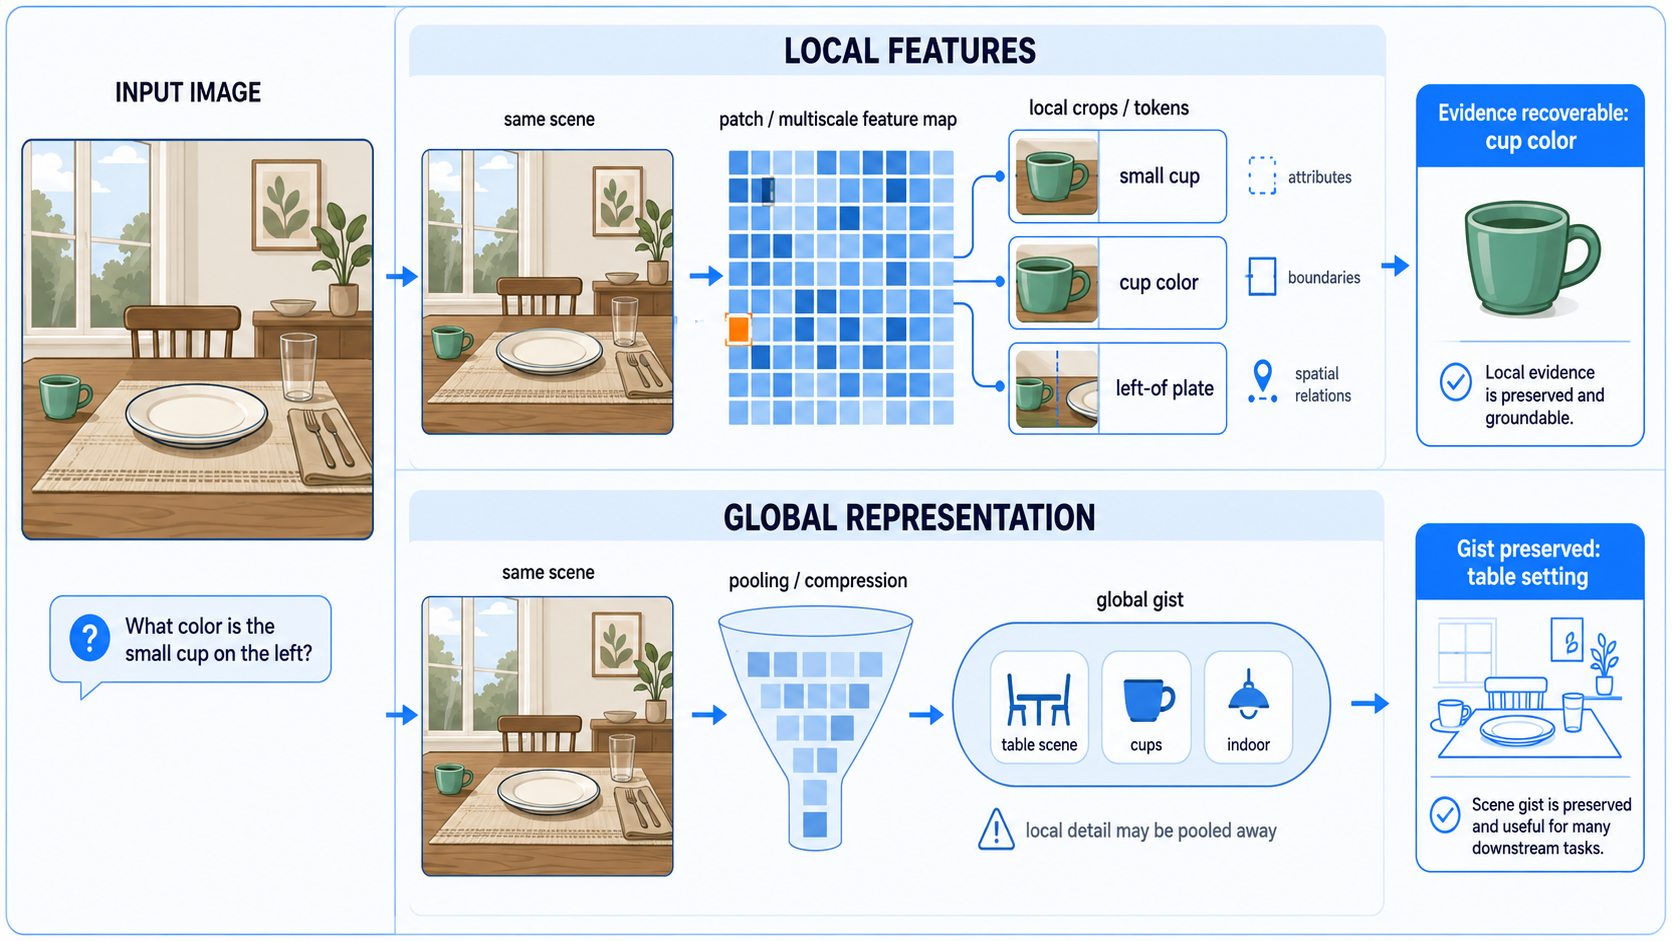
\includegraphics[width=0.96\textwidth]{figures/ch23/fig_local_detail_global_representation.png}
\caption{\textbf{Local detail versus global representation.} Patch-level or multiscale features can preserve small objects, attributes, and spatial relations. A pooled representation may preserve the scene gist while discarding the local evidence needed for grounding.}
\label{fig:ch23-local-detail-global-representation}
\end{figure}

\subsection{How Pretraining Shapes What Survives}

The visual encoder learns its representation from an objective. Different objectives reward different information.

\paragraph{Supervised pretraining.} The classic recipe is image-to-class-label learning. It can produce strong category recognition, but labels are coarse. The encoder may focus on discriminative class features and ignore details that do not help classification. A classifier can recognize ``dining room'' without preserving the exact color of a small cup.

\paragraph{Masked image modeling.} BEiT-style pretraining hides patches and predicts discrete visual tokens; MAE-style pretraining hides many patches and reconstructs pixels or patch content~\cite{bao2021beit,he2022masked}. These objectives encourage the model to learn image structure without manual labels. They can preserve useful spatial and local regularities. But reconstruction is not the same as semantic understanding, and pixel fidelity is not identical to reasoning usefulness.

\paragraph{Self-distillation and self-supervised features.} DINO-style methods train stable representations across views and augmentations; DINOv2-style systems show that vision-only self-supervision can produce strong general-purpose features~\cite{oquab2023dinov2}. These representations can transfer well, but they are still not language-aligned by themselves.

\paragraph{Dense and region-aware pretraining.} Segmentation-oriented encoders and region-level systems emphasize object masks, boundaries, and dense spatial evidence. Segment Anything is important here not because this chapter is a segmentation chapter, but because it makes region-level evidence visible as a first-class visual representation~\cite{kirillov2023segment}.

\begin{center}
\small
\begin{tabularx}{\textwidth}{@{}p{3.6cm}p{5.3cm}X@{}}
\toprule
\textbf{Objective} & \textbf{What it rewards} & \textbf{What it may ignore} \\
\midrule
Supervised classification & Class-discriminative features & Fine attributes; small objects \\
Masked reconstruction & Local structure, pixels, or patch content & Semantic task relevance \\
Self-distillation & Invariant object and scene features & Exact text; rare details \\
Segmentation / region-level & Boundaries, masks, and regions & Language semantics \\
Contrastive image-text & Global semantic matching & Local grounding; Chapter~\ref{ch:cross-modal-alignment} studies this directly \\
\bottomrule
\end{tabularx}
\end{center}

\begin{tcolorbox}[colback=gray!8, colframe=gray!40, title=\textbf{Cross-Chapter Echo: Evidence Before Explanation}]
Chapter~\ref{ch:long-context-retrieval-memory} warned that a RAG answer can fail because the right paragraph was never retrieved. The visual analogue is a VLM answer that fails because the right pixels never became recoverable visual tokens. In both cases, later reasoning is downstream of evidence exposure.
\end{tcolorbox}

\subsection{Vision-Only Is Not Language Grounding}

Vision-only pretraining can produce strong visual representations. It can learn shapes, textures, objects, boundaries, and spatial regularities. It does not by itself solve the language grounding problem. A feature may separate cups from plates without making the phrase ``the small cup on the left'' easy for an LLM to address. Chapter~\ref{ch:cross-modal-alignment} will study how visual representations acquire language-addressable meaning through image-text pairs and contrastive objectives.

The boundary is important. This chapter asks what visual information is encoded. The next chapter asks how those representations line up with words, captions, and concepts.

\begin{quickrecap}
\textbf{Quick Recap.}
\begin{itemize}[nosep,leftmargin=1.5em]
  \item Visual encoders produce learned representations, not raw images.
  \item Local features support attributes, boundaries, small objects, and spatial questions; global features support scene gist and image-level matching.
  \item Pretraining objectives shape which details survive.
  \item Vision-only pretraining can be powerful without making features language-addressable.
\end{itemize}
\textit{Next: resolution and patch size turn visual representation into a token-budget problem.}
\end{quickrecap}


%----------------------------------------------------------------------
\section{Resolution, Token Budget, and Detail Preservation}
\label{sec:ch23-resolution-token-budget}

Resolution is not a free accuracy knob. It is a token-budget decision.

For fixed patch size, increasing resolution increases $N_v$ quadratically. For fixed resolution, decreasing patch size also increases $N_v$ quadratically. The system receives more visual evidence, but it pays with compute, memory, latency, and downstream interface pressure.

\begin{figure}[t]
\centering
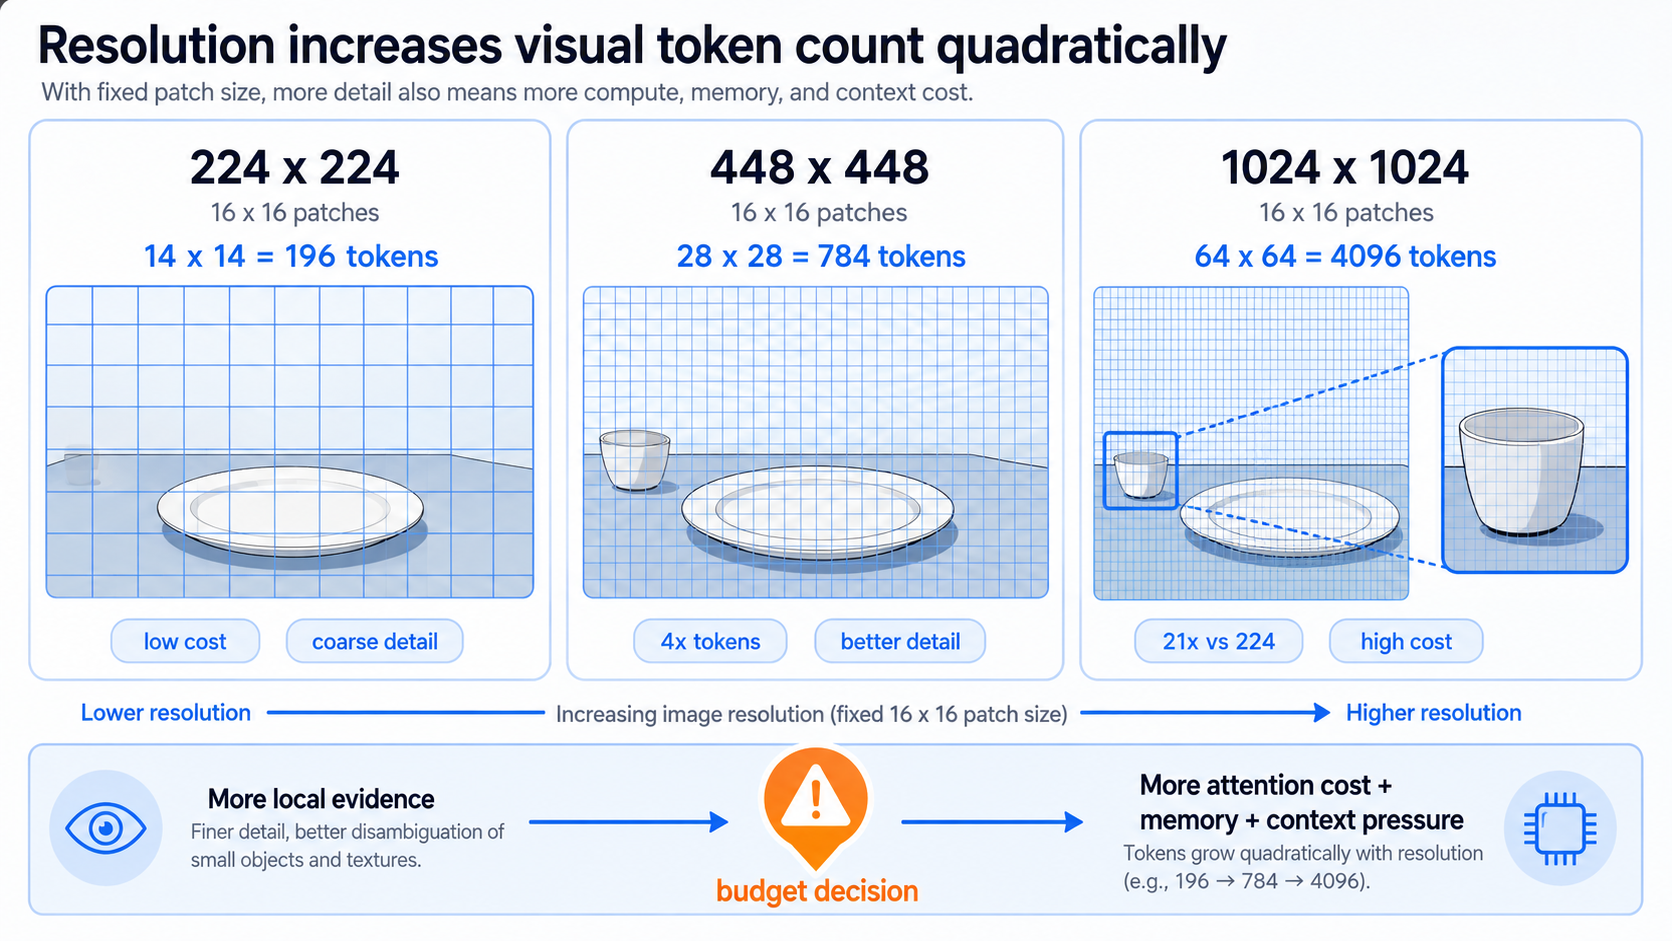
\includegraphics[width=0.96\textwidth]{figures/ch23/fig_resolution_token_budget.png}
\caption{\textbf{Resolution is a visual token budget.} With fixed $16 \times 16$ patches, $224 \times 224$ produces 196 visual tokens, $448 \times 448$ produces 784, and $1024 \times 1024$ produces 4096. Detail preservation competes with attention cost and context budget.}
\label{fig:ch23-resolution-token-budget}
\end{figure}

\subsection{Patch Size and Image Resolution}

Patch size controls granularity. Larger patches are cheaper but coarser. Smaller patches can preserve boundaries, text, and small objects, but increase token count. The same small cup can be a visible object in an $8 \times 8$ patch system and a faint mixture inside one $16 \times 16$ patch after downsampling.

Image resolution controls how many pixels reach the encoder before patching. Downsampling can erase small details. Upsampling cannot recover detail that was not present in the input, but feeding a higher-resolution original may keep small objects large enough to occupy multiple patches.

\begin{tcolorbox}[colback=blue!5, colframe=blue!40, title=\textbf{Pause and Verify}]
A small object occupies $12 \times 12$ pixels in a $1024 \times 1024$ image. The system resizes the image to $224 \times 224$ before using $16 \times 16$ patches. What might go wrong?

\medskip
\noindent\textbf{Reasoning.} The object shrinks by a factor of $224/1024 \approx 0.22$, so it becomes roughly $2.6 \times 2.6$ pixels. It may occupy only a tiny fraction of one patch. The encoder may not preserve its color, boundary, or identity. A later grounding error may therefore originate in visual tokenization rather than language reasoning.
\end{tcolorbox}

\subsection{Global View Plus Local Crops}

One common design pattern is:

\[
\text{global low-resolution view} + \text{high-resolution local evidence}.
\]

The global view gives scene context. Local crops preserve details. For the running example, a low-resolution full image may show a table scene but lose the small cup's color. A crop of the left side may make the cup large enough to answer.

This is visual context engineering. Chapter~\ref{ch:long-context-retrieval-memory} studied a textual pattern: read broad context cheaply, then spend tokens on high-value evidence. High-resolution vision has the same shape. The system must decide which visual evidence deserves expensive tokens.

\subsection{Visual Token Compression and Selection}

Modern systems do not always pass every visual token forward. They may pool, merge, prune, resample, or select tokens under a budget. Token merging reduces redundant patches. Adaptive pruning removes low-salience tokens. Perceiver-style compressors can map a large input set to a fixed number of latent tokens. Dynamic-resolution systems can pack images of different sizes or process selected crops at higher detail. NaViT-style approaches make variable-resolution patch sequences easier to batch and train~\cite{dehghani2023patch}. Token merging methods such as ToMe illustrate the broader compression pressure~\cite{bolya2023token}.

\begin{figure}[t]
\centering
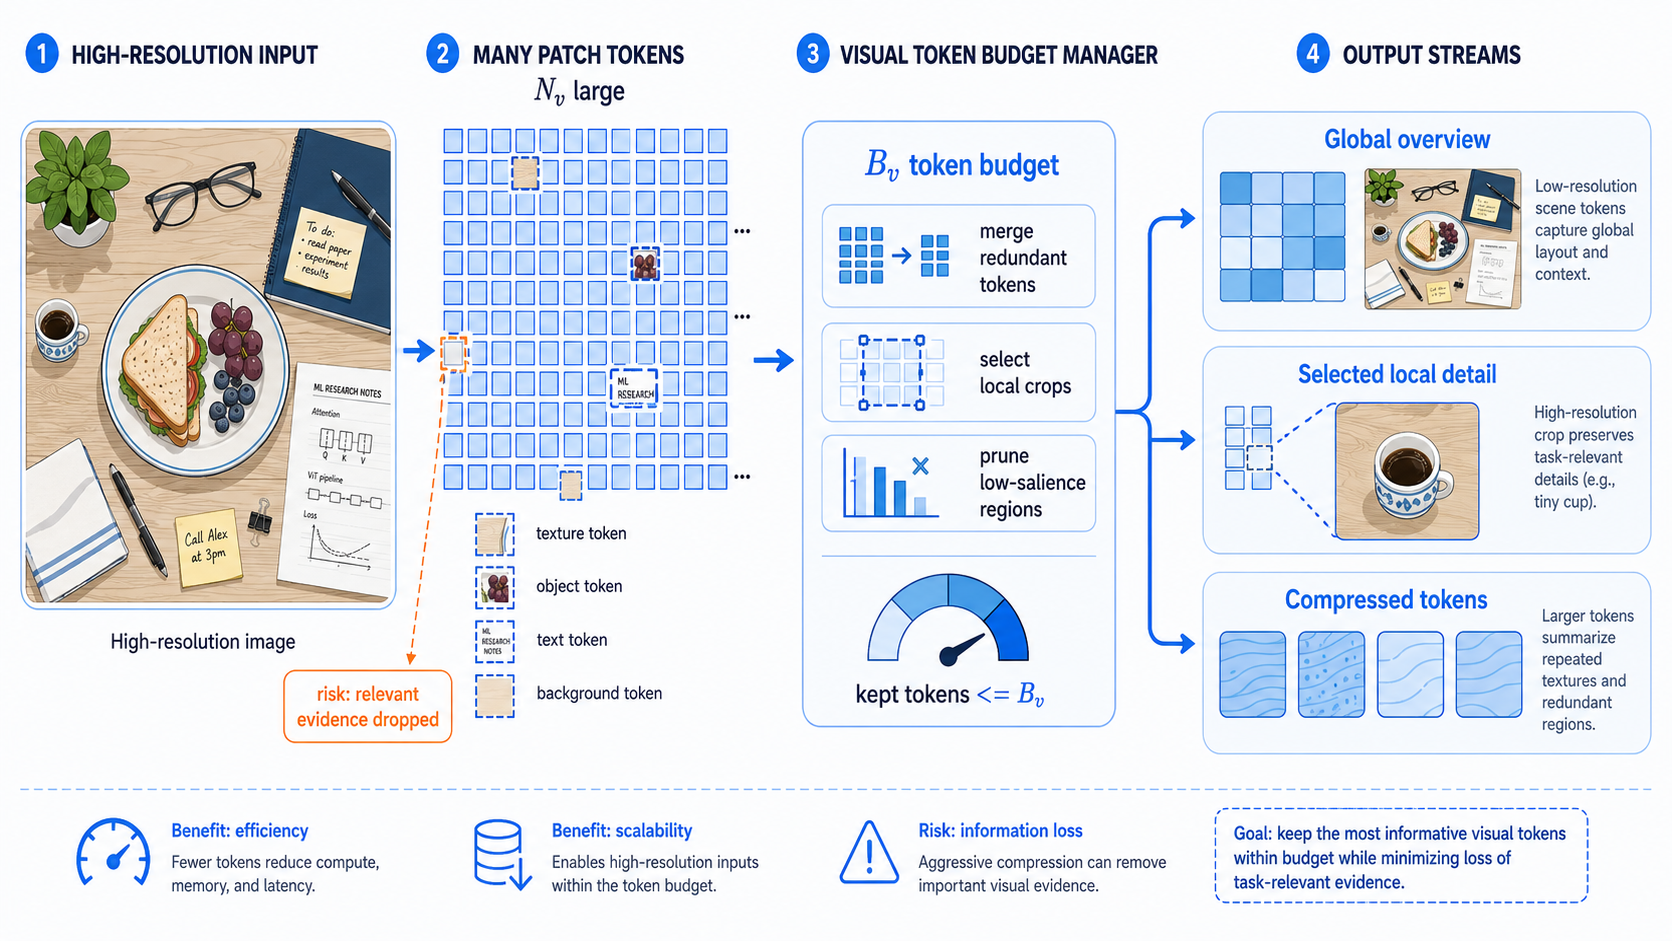
\includegraphics[width=0.96\textwidth]{figures/ch23/fig_dynamic_visual_token_selection.png}
\caption{\textbf{Dynamic visual token selection.} High-resolution encoders often manage a visual token budget by combining a global overview with selected local detail, compressed tokens, or pruned low-salience regions. The gain is efficiency; the risk is dropping task-relevant evidence.}
\label{fig:ch23-dynamic-token-selection}
\end{figure}

Compression is not neutral. If the selection policy keeps the central plate and removes the small left cup, the downstream LLM cannot recover the answer. If the policy keeps a local crop around the cup, the same model may succeed. This makes token selection an attribution layer, not just an efficiency trick.

\begin{tcolorbox}[colback=blue!5, colframe=blue!40, title=\textbf{More Pixels Are Not Always More Evidence}]
Higher resolution can help, but it is not a universal fix. More visual tokens can force stronger compression at the interface, introduce distracting local detail, or make the system choose fewer repeated checks under a fixed cost budget. Crops can preserve local detail while losing global context. Positional interpolation and aspect-ratio changes can also alter spatial relations. The right question is not ``more pixels?'' but ``which visual evidence should receive the expensive tokens?''
\end{tcolorbox}

\begin{tcolorbox}[colback=orange!5, colframe=orange!60, title=\textbf{For Project~5: Encoding Experiments}]
When building the controlled VLM grounding benchmark, record visual input conditions:
\begin{itemize}[nosep,leftmargin=1.5em]
  \item full image resolution and any resized resolution;
  \item patch size or approximate visual token count when available;
  \item full-image versus crop condition;
  \item whether a small object question becomes answerable after enlargement;
  \item whether failures are stable across repeated runs or resolution settings.
\end{itemize}
Before blaming hallucination, test whether the visual evidence was visible to the encoder.
\end{tcolorbox}

\begin{quickrecap}
\textbf{Quick Recap.}
\begin{itemize}[nosep,leftmargin=1.5em]
  \item Higher resolution and smaller patches preserve detail but increase visual tokens.
  \item Global overview plus local crops is the visual analogue of context routing.
  \item Token compression, pruning, and selection manage budget but can drop task-relevant evidence.
  \item High-resolution perception is context engineering in visual form.
\end{itemize}
\textit{Next: the same budget choices explain many encoding-layer failure modes.}
\end{quickrecap}


%----------------------------------------------------------------------
\section{What Visual Tokens Preserve and Lose}
\label{sec:ch23-preserve-lose}

When a VLM answers incorrectly, not every error is a reasoning error. The answer may fail because the relevant visual evidence was never encoded. This section names common encoding-layer failures so later chapters can separate perception, interface, binding, and reasoning mistakes.

\subsection{Failure Modes at the Encoding Layer}

\paragraph{Small-object loss.} An object occupies too few pixels after resizing or too small a fraction of a patch. It disappears into background features.

\paragraph{Attribute loss.} Color, texture, fine shape, text, or material detail is not represented clearly enough. The model may know that an object exists without preserving the attribute needed by the question.

\paragraph{Boundary loss.} A patch mixes object and background, or two adjacent objects share the same coarse feature. Localization becomes ambiguous.

\paragraph{Spatial precision loss.} The encoder preserves the scene category but not precise left/right, above/below, inside/outside, or near/far relations.

\paragraph{Pooling loss.} A global embedding preserves image gist while discarding local details. This is common when the representation was optimized for image-level matching.

\paragraph{Salience bias.} Large, central, common objects dominate the representation. Small, peripheral, rare, or low-contrast objects receive weaker features.

\paragraph{Resolution mismatch.} The model was trained under one resolution or patch grid and used under another. Positional interpolation, token selection, and scale assumptions may change behavior.

\subsection{The Running Example Revisited}

For ``What color is the small cup on the left?'', these failures look different:

\begin{itemize}[nosep,leftmargin=1.5em]
  \item If downsampling turns the cup into three pixels, the object may be lost.
  \item If the cup is visible but its color is blurred with the table, the attribute is lost.
  \item If one patch contains both cup and plate, the boundary is mixed.
  \item If a pooled representation says ``table setting'' but no token preserves the cup, local evidence was pooled away.
  \item If token pruning keeps the central plate and removes the left edge, salience bias won.
\end{itemize}

The important habit is not to excuse every VLM mistake as perception. It is to localize the first plausible broken layer. If a high-resolution crop still fails, the problem may lie in alignment, interface, binding, instruction following, or language reasoning. If the crop fixes the answer, the full-image failure probably began in encoding, salience, or budget.

\begin{figure}[t]
\centering
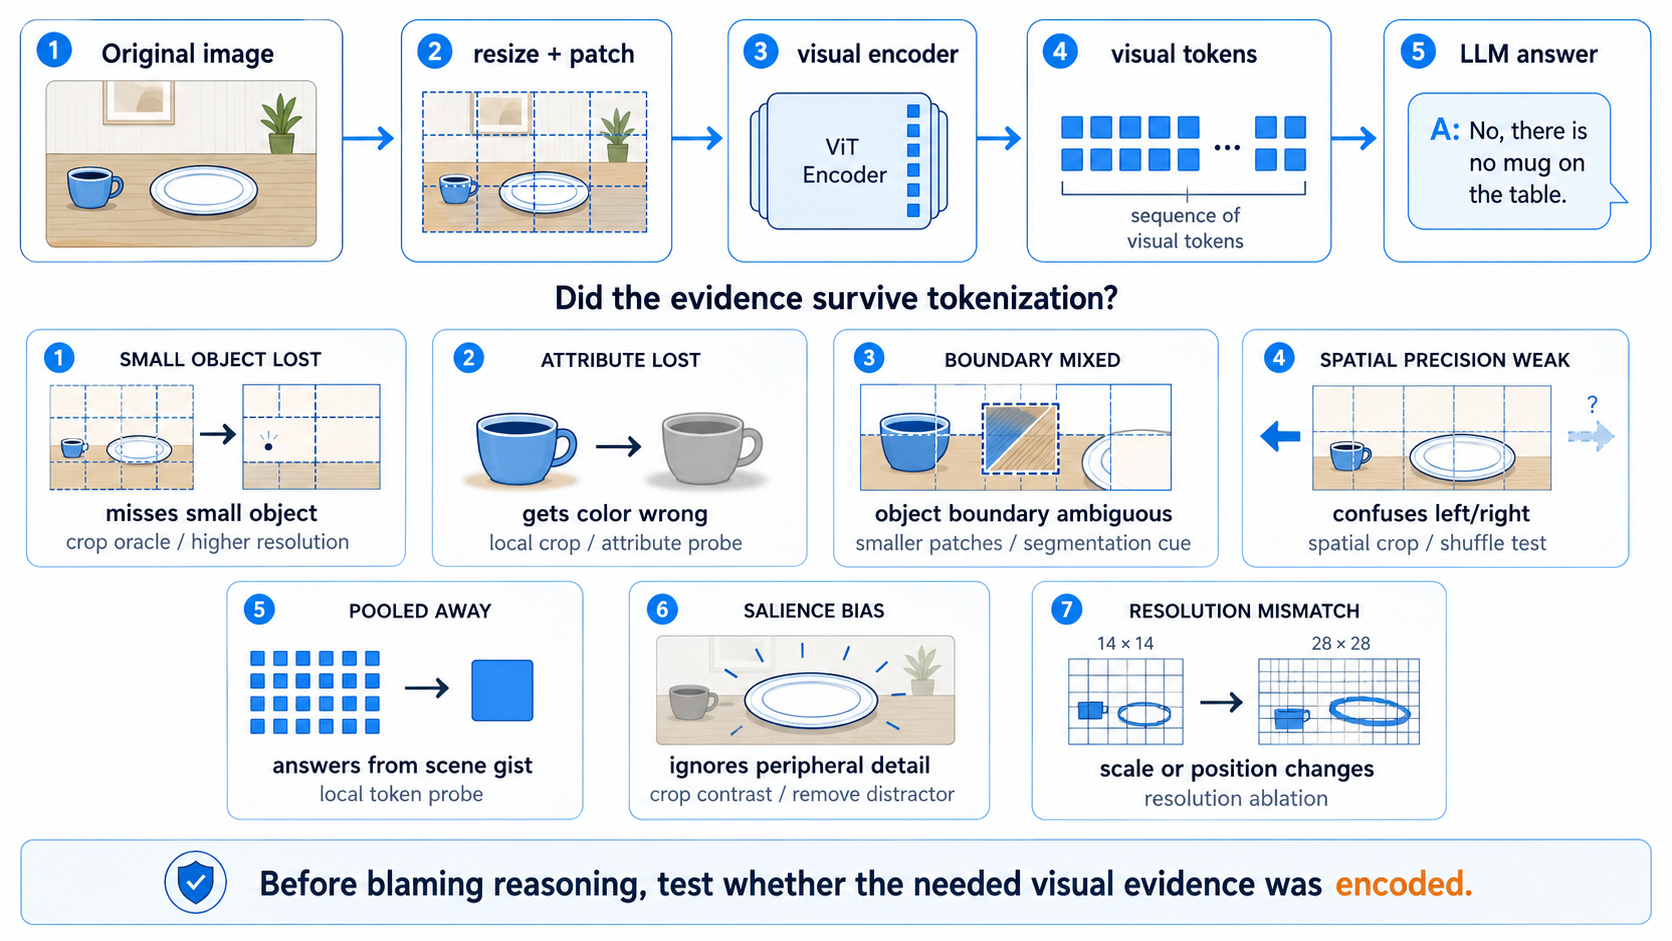
\includegraphics[width=0.96\textwidth]{figures/ch23/fig_encoding_failure_audit.png}
\caption{\textbf{Encoding failure audit.} Many VLM symptoms can originate before language generation: small objects disappear, attributes blur, boundaries mix, spatial precision weakens, local details are pooled away, salience bias dominates, or resolution mismatch changes the representation.}
\label{fig:ch23-encoding-failure-audit}
\end{figure}

\subsection{A Ch23-Level Failure Table}

Text in images appears in this table only as an example of fine visual detail loss. OCR, document understanding, screenshots, and GUI agents require additional machinery and are outside this chapter's scope.

\begin{center}
\small
\begin{tabularx}{\textwidth}{@{}p{3.0cm}p{5.1cm}X@{}}
\toprule
\textbf{Symptom} & \textbf{Possible Ch23-level cause} & \textbf{Diagnostic} \\
\midrule
Misses small object & Object lost after resizing or patching & Crop oracle; higher-resolution input \\
Gets color wrong & Attribute not preserved in local features & Local crop; attribute probe \\
Confuses left/right & Spatial precision or positional representation weak & Spatial crop/shuffle test \\
Counts incorrectly & Instances not separately represented & Resolution ablation; region proposals \\
Ignores text in image & OCR-like detail lost before language stage & High-resolution crop; OCR tool comparison \\
Answers from scene prior & Global semantics dominate local evidence & Local evidence contrast; remove distractors \\
\bottomrule
\end{tabularx}
\end{center}

\begin{quickrecap}
\textbf{Quick Recap.}
\begin{itemize}[nosep,leftmargin=1.5em]
  \item Visual failures can begin before alignment, prompting, or language reasoning.
  \item Small objects, attributes, boundaries, spatial relations, and local details are vulnerable to patching, resizing, pooling, and pruning.
  \item A useful failure audit asks whether the evidence was recoverable from visual tokens before blaming the LLM.
\end{itemize}
\textit{Next: diagnostics turn this failure taxonomy into tests.}
\end{quickrecap}


%----------------------------------------------------------------------
\section{Diagnostics for Visual Encoders}
\label{sec:ch23-visual-encoder-diagnostics}

This chapter is not a full evaluation chapter, but it should leave you with practical diagnostics. The goal is to separate three claims:

\begin{enumerate}[nosep,leftmargin=1.5em]
  \item The visual evidence was not encoded clearly.
  \item The evidence was encoded but not aligned or routed to the language model.
  \item The evidence reached the model, but the model failed to bind, reason, or answer.
\end{enumerate}

Chapter~\ref{ch:evaluating-model-systems} called this habit attribution. Here the attribution target is the visual encoder.

\subsection{The Visual Encoding Diagnostic Ladder}

Use diagnostics in an order that moves from cheapest calibration to stronger component attribution:

\begin{enumerate}[leftmargin=1.5em]
  \item \textbf{Human-visible evidence check.} Show the image at the model's actual input resolution. If a human cannot answer, the input may not contain enough evidence.
  \item \textbf{Same image at model input resolution.} Inspect the resized, cropped, padded, or tiled version that actually enters the image processor.
  \item \textbf{Higher-resolution ablation.} Increase resolution or use a system with finer patch granularity and test whether the answer changes.
  \item \textbf{Crop oracle.} Provide a crop known to contain the relevant evidence.
  \item \textbf{Contrast or counterfactual image.} Change the local evidence while holding the scene mostly fixed.
  \item \textbf{Visual probe.} Test whether the object, attribute, or relation is recoverable from visual tokens.
  \item \textbf{Downstream interface test.} If the evidence is recoverable from visual tokens but not used in answers, Chapter~\ref{ch:visual-language-interface} and Chapter~\ref{ch:grounding-binding-visual-reasoning} become the next attribution targets.
\end{enumerate}

The ladder does not prove causality by itself. It helps locate the first layer where the explanation becomes plausible.

\subsection{Resolution and Patch Granularity Ablations}

Run the same image at multiple resolutions or with systems that use different patch sizes. If the answer appears only at higher resolution, the bottleneck may be visual detail. If higher resolution does not help, the failure may lie elsewhere.

This test should report cost as well as success. A $1024 \times 1024$ input with $16 \times 16$ patches produces 4096 visual tokens before any additional crops. That may be reasonable for a high-value medical image and unreasonable for a low-stakes chat request. Cost per useful visual answer depends on task value and failure cost, not on accuracy alone.

\subsection{Crop Oracle and Global-Local Comparison}

A crop oracle gives the system a region known to contain the relevant evidence. If the crop succeeds while the full image fails, the problem may be salience, resolution, token budget, or visual search. If the full image succeeds but the crop fails, the question may require global context. If both fail, the issue may be attribute representation, language alignment, interface routing, or reasoning.

For the small-cup example, test:

\begin{itemize}[nosep,leftmargin=1.5em]
  \item full image at standard resolution;
  \item full image at higher resolution;
  \item left-side crop containing the cup;
  \item crop enlarged so the cup occupies many patches;
  \item contrast image where the cup color changes while the scene stays similar.
\end{itemize}

\subsection{Visual Probes and Salience Inspection}

Visual probing asks whether an object, attribute, or relation is recoverable from visual tokens using a simple classifier or diagnostic head. A positive probe does not prove the language model will use the feature. A negative probe is stronger evidence that the feature may not be represented in an accessible way.

Attention maps and token-salience visualizations can be useful, but they are suggestive rather than decisive. A highlighted patch is not proof of causal use. A low-salience patch is not proof of irrelevance. Treat these tools as debugging aids, not explanations by themselves.

\subsection{Human-Visible Evidence Check}

One simple diagnostic is often overlooked: show a human the image at the model's actual input resolution. If a human cannot answer after the same downsampling, the model may not have had enough visual evidence. If a human can answer easily from the downsampled image, the failure is less likely to be pure resolution loss.

This check prevents unfair expectations. It also prevents the opposite mistake: blaming resolution when the evidence was visible but the system failed to use it.

\begin{tcolorbox}[colback=orange!5, colframe=orange!60, title=\textbf{For Project~5: Report Template Additions}]
For each controlled VLM grounding example, include:
\begin{itemize}[nosep,leftmargin=1.5em]
  \item original image size and model input size;
  \item estimated visual-token budget if known;
  \item task type: small object, attribute, spatial relation, counting, text, or distractor;
  \item full-image result, crop-oracle result, and high-resolution result;
  \item whether repeated runs produce the same failure;
  \item best explanation: encoding failure, interface failure, binding failure, or reasoning failure.
\end{itemize}
\end{tcolorbox}

\begin{quickrecap}
\textbf{Quick Recap.}
\begin{itemize}[nosep,leftmargin=1.5em]
  \item Resolution ablations test whether more visual detail changes the answer.
  \item Crop oracles test whether the system can answer when relevant evidence is made salient.
  \item Probes and salience maps are useful but not definitive.
  \item Human-visible evidence checks calibrate whether the model's input contained enough information.
\end{itemize}
\textit{Next: we distill the image-as-token lesson and hand off to cross-modal alignment.}
\end{quickrecap}


%----------------------------------------------------------------------
\section{Summary: The Image-as-Token Lesson}
\label{sec:ch23-summary}

Chapter~23 established that multimodal modeling begins with visual tokenization. Images are not naturally token sequences. Visual encoders create sequences by resizing, patching, embedding, adding position, pooling, compressing, and sometimes selecting visual evidence. These choices determine which details are available to later alignment, interface, instruction tuning, and reasoning stages.

The main lesson is not that higher resolution is always better or that one encoder family solves perception. It is that visual evidence enters a model through a budgeted representation. A model may fail because it reasoned poorly. It may also fail because a small object, color, boundary, word, or spatial relation never survived the encoder.

\begin{takeaways}
\begin{enumerate}[nosep]
  \item A VLM does not see pixels directly; it sees learned visual tokens.
  \item Patch size and image resolution determine the first visual-token budget.
  \item Doubling image resolution roughly quadruples patch-token count for fixed patch size.
  \item Local and global visual representations support different tasks.
  \item Vision-only pretraining can learn strong features without making them language-addressable.
  \item High-resolution perception is context engineering in visual form.
  \item Visual failure attribution starts by asking whether the evidence survived tokenization.
\end{enumerate}
\end{takeaways}

\section*{Summary}

\paragraph{What this chapter established.} We turned the phrase ``the model saw the image'' into a technical question. Which version of the image did the model see? At what resolution? Through which patching scheme? With which positional encoding? Under what token budget? With which details preserved, pooled, pruned, or lost? Those questions define the first audit layer of Part~V.

\paragraph{The image-as-token lesson.} The central abstraction of this chapter is not the pixel and not the caption. It is the visual token: a learned, budgeted representation of a region or compressed set of regions. Once images become tokens, they inherit the strengths and limits of sequence models. They can be attended to, routed, compressed, and aligned. They can also drop small details, blur attributes, weaken spatial precision, and spend context budget quickly.

\paragraph{One sentence.} A VLM's visual reasoning is only as good as the visual evidence that survives tokenization.

\paragraph{What comes next.} Chapter~\ref{ch:cross-modal-alignment} asks how visual representations acquire language-addressable meaning. A visual encoder can produce useful features, but a multimodal foundation model also needs those features to align with words, captions, and concepts.

\section*{Key Equations}

\begin{center}
\begin{tabularx}{\textwidth}{@{}lX@{}}
\toprule
\textbf{Equation} & \textbf{Meaning} \\
\midrule
$V = f_v(I)$ & A visual encoder maps an image to a visual token sequence or representation. \\
$N_v = (H/P)(W/P)$ & For non-overlapping square patches, visual-token count grows with image area and shrinks with patch area. \\
$N_{\mathrm{total}} \approx N_{\mathrm{global}} + \sum_j N_{\mathrm{crop},j}$ & Multi-crop systems spend visual tokens on a global view plus selected local evidence. \\
$B_v \geq N_{\mathrm{kept}}$ & A downstream interface can only use the visual tokens that fit its budget after selection, pooling, or compression. \\
\bottomrule
\end{tabularx}
\end{center}

\section*{Key Readings}

\begin{itemize}[leftmargin=1.5em]
  \item Dosovitskiy et al., ``An Image is Worth 16x16 Words''~\cite{dosovitskiy2020image}. Read for the patch-token formulation that made ViTs central to multimodal pipelines.
  \item He et al., ``Masked Autoencoders Are Scalable Vision Learners''~\cite{he2022masked}. Read for masked image modeling as scalable vision-only pretraining.
  \item Bao et al., ``BEiT''~\cite{bao2021beit}. Read for discrete visual token prediction as a BERT-like image pretraining objective.
  \item Liu et al., ``Swin Transformer''~\cite{liu2021swin}. Read for hierarchical and windowed visual attention under locality and resolution constraints.
  \item Oquab et al., ``DINOv2''~\cite{oquab2023dinov2}. Read for strong self-supervised visual features that transfer beyond narrow labels.
  \item Kirillov et al., ``Segment Anything''~\cite{kirillov2023segment}. Read selectively for dense visual representation and the importance of region-level evidence.
  \item Dehghani et al., ``Patch n' Pack''~\cite{dehghani2023patch}. Read for dynamic-resolution visual tokenization and packing pressure in high-resolution vision.
\end{itemize}

\flushbottom
